%***********************************************************************
% Lab Report Template
% R. W. Melton
% May 19, 2019
% August 24, 2020
%***********************************************************************
%Modify the following macros to set document property values
%used for cover sheet (title page) and page header
\newcommand{\CourseNumber}{CMPE-250}
\newcommand{\CourseName}{Assembly and Embedded Programming}
\newcommand{\SemesterName}{Fall 2020}
\newcommand{\SemesterCode}{20201}
\newcommand{\LabExNum}{2}
\newcommand{\LabExTitle}{Basic Arithmetic Operations}
\newcommand{\StudentName}{Andrei Tumbar}
\newcommand{\DateSubmit}{09-14-20}
\newcommand{\LabSection}{5}
\newcommand{\LabInstructor}{Melton}
\newcommand{\TAa}{Tianran Cui}
\newcommand{\TAb}{Anthony Bacchetta}
\newcommand{\LectureSection}{1}
\newcommand{\LectureInstructor}{Melton}
%End macros for document property values
%***********************************************************************
\title{Lab Ex. \LabExNum\ Report}
\author{\StudentName}
\date{\DateSubmit}
\makeatletter %make \title, \author, and \date availabile with \@
\newcommand{\FontSize}{12}
\newcommand{\FontUnit}{pt}
\newcommand{\HeadSize}{\dimexpr \FontSize\FontUnit + 2pt \relax}
\documentclass[\FontSize\FontUnit,letterpaper,oneside]{article}
\usepackage[twoside=false,margin=1in]{geometry}
\usepackage[utf8]{inputenc}
\usepackage[USenglish]{babel}
\usepackage{graphicx}
\usepackage[normalem]{ulem}
\usepackage{newtxtext, newtxmath}
%If newtx package had to be installed in multiuser environment
%regular user may have to run updmap command to avoid following error
%FATAL:  ``PK font ts1-qtmr could not be created.'' in miktex-makepk
%Alternatively, uncomment the following line
%\pdfmapfile{=pdftex35.map
\usepackage{booktabs}
\usepackage{enumitem}
\usepackage{nameref}
\usepackage[pdfborder={0 0 0},plainpages=false,pdfpagelabels]{hyperref}
\def\code#1{\texttt{#1}}
%If hyperref generates errors on first build, rebuild.            
\hypersetup{pdfauthor={\@author},
            pdftitle={\@title},
            pdfsubject={\CourseNumber\ \SemesterCode},
            %pdfkeywords={},
            %pdfproducer={Latex with hyperref, or other system},
            %pdfcreator={pdflatex, or other tool}
            urlcolor=none}
\setlength{\topsep}{\z@}
\setlength{\partopsep}{\z@}
\setlength{\itemsep}{\z@}
\setlength{\parindent}{\z@}
\setlength{\parskip}{\FontSize\FontUnit plus 2pt minus 1pt}
\setlength{\baselineskip}{\dimexpr \FontSize\FontUnit + 2pt \relax}
\renewcommand \baselinestretch{1}
\makeatletter
  \renewcommand \section{
    \@startsection{section}{1}{\z@}
      %Before 2 lines, accounting for normal \parskip
      {\dimexpr \FontSize\FontUnit * 2 - \parskip \relax plus 0pt minus 0pt}
      %After 1 line, accounting for normal \parskip
      {0.1pt plus 2pt minus 1pt} %nonzero amount to get normal \parskip
      {\normalfont\normalsize\bfseries}} 
  \renewcommand \subsection{
    \@startsection{paragraph}{2}{\z@}
      %Before 1 lines, accounting for normal \parskip
      {0.1pt plus 2pt minus 1pt}
      %After 0.5 em on same line as heading
      {-0.5em} 
      {\normalfont\normalsize\bfseries}} 
  \renewcommand \subsubsection{
    \@startsection{paragraph}{3}{\z@}
      %Before 1 line, accounting for normal \parskip
      {0.1pt plus 2pt minus 1pt}
      %After 0.5 em on same line as heading
      {-0.5em} 
      {\normalfont\normalsize\uline}} 
  \renewcommand \paragraph{
      \@startsection{paragraph}{4}{\z@}
      %Before 1 line, accounting for normal \parskip
      {0.1pt plus 2pt minus 1pt}
      %After 0.5 em on same line as heading
      {-0.5em} 
      {\normalfont\normalsize}} 
\makeatother
\pagenumbering{arabic}
\headheight=\HeadSize
\usepackage{fancyhdr}
\renewcommand{\headrulewidth}{0pt}
\renewcommand{\footrulewidth}{0pt}
\makeatletter %make \title, \author, and \date availabile with \@
\pagestyle{fancy}
\fancyhead{} %clear all header fields
\fancyhead[L]{\small \CourseNumber\ \SemesterCode \@author:  \@title}
\fancyhead[R]{\small Page \thepage\ of \pageref*{LastPage}}
\fancyfoot{} %clear all footer fields
\fancypagestyle{plain}{
  \renewcommand{\headrulewidth}{0pt}
  \renewcommand{\footrulewidth}{0pt}
  \fancyhf{} %clear header and footer fields
  \fancyfoot[C]{\small \CourseNumber\ \SemesterCode\ \@author:  \@title:  
    Page \thepage\ of \pageref*{LastPage}}
}
%May require second build to get correct page numbers.            
\begin{document}
\raggedbottom
\widowpenalties 1 10000
\lefthyphenmin=4
\righthyphenmin=4
\setlist{nolistsep}
%***********************************************************************
%Title page is automatically generated from macros at top of file
\pagenumbering{roman}
\begin{titlepage}
  %No space before paragraph at top of page
  %\vspace{\dimexpr-2\parsep-2\parskip\relax}
  %1.5 in before center (list) at top of page
  \vspace*{\dimexpr 1.5in - \topsep - \partopsep - \topskip - \parskip \relax}
  \begin{center}
    \textbf{\large\CourseNumber\ \CourseName\linebreak
      \linebreak
      Laboratory Exercise \LabExNum\linebreak
      \linebreak
      \LabExTitle}
  \end{center}
  \vspace*{\dimexpr 1.5in - \topsep - \partopsep - \topskip \relax}
  \par By submitting this report, I attest that its contents are wholly 
    my individual writing about this exercise and that they reflect 
    the submitted code.  I further acknowledge that permitted 
    collaboration for this exercise consists only of discussions of 
    concepts with course staff and fellow students.  Other than code 
    provided by the instructor for this exercise, all code was 
    developed by me.
  \null
  \vspace*{4\parskip}
  \hspace*{3.25in}\begin{tabular}[t]
    {@{\hskip0pt}r    %Specification
     @{\hskip1em}l    %Value
     @{\hskip0pt}}
    \toprule[1pt]
    \multicolumn{2}{l}{\StudentName}\\
    \multicolumn{2}{l}{\DateSubmit}\\
    \\
    Lab Section:&\LabSection\\
    Instructor:&\LabInstructor\\
    TA:&\TAa\\
    &\TAb\\
    \\
    Lecture Section:&\LectureSection\\
    Lecture Instructor:&\LectureInstructor
  \end{tabular}
\end{titlepage}
\pagenumbering{arabic}
\thispagestyle{plain}
%***********************************************************************
%Report body begins here
\section*{Results}

Screen captures were taken for two different input sets. The variable memory
is divided into 4-byte signed decimal values. The first two values are \code{P}
and \code{Q}. The next three are \code{F}, \code{G}, and \code{Result} respectively. 

\begin{figure}[h!]
	\centering
	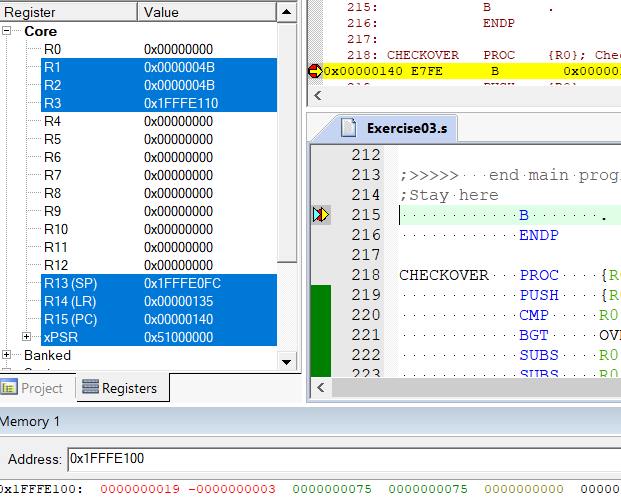
\includegraphics[]{capture-1}
	\caption{Debugger results after program execution with first input set.}
	\label{fig:capture1}
\end{figure}

Figure \ref{fig:capture1} shows the register values and memory contents after
execution with the first input set where $P = 19_{10}$ and $Q=-3_{10}$

\pagebreak

\begin{figure}[h!]
	\centering
	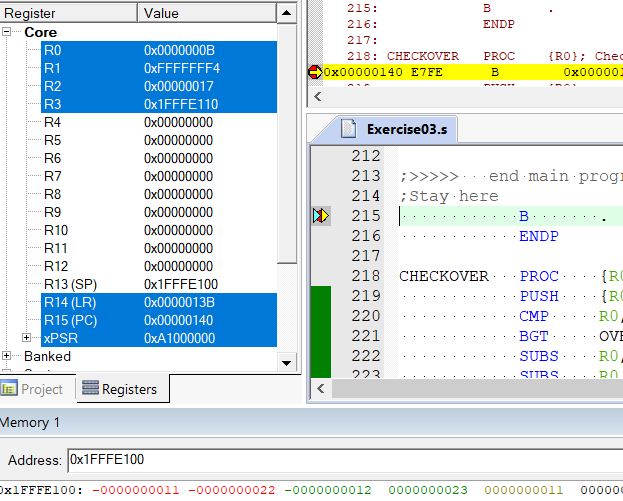
\includegraphics[]{capture-2}
	\caption{Debugger results after program execution with second input set.}
	\label{fig:capture2}
\end{figure}

Figure \ref{fig:capture2} shows the register values as well as memory contents
after the second input set where $P = -11_{10}$ and $Q=-22_{10}$.

According to prelab calculations, in the first input set \code{F} and \code{G}
should both be $75_{10}$ which would case \code{Result} to overflow. Figure
\ref{fig:capture1} shows the \code{Result} variable with a value of $10$
and \code{F} and \code{G} both have $75_{10}$ indicating that the results were
correct.

Similarly, for the second input set, prelab calculations revealed $F=-12_{10}$,
$G=23_{10}$, and $Result=11_{10}$. This is corroborated by the results shown in
Figure \ref{fig:capture2}.

\section*{Question}
In theory you could reduce the overflow of the calculations if the overflow
occurs in one of the intermediate steps. For example in the expression $G=3P - 2Q + 12$, $G$ would overflow if $3P$ was out of range of $[-128,127]$ even the final
result could still be within that range. To reduce this overflow, the order of
operations can be changed like so:

\begin{equation}
G = P + 2 \cdot (P - Q) + 12
\end{equation}

This alternate equation would stop overflow in intermediate steps but would obviously not avoid it if the result were to overflow.

\label{LastPage}
\end{document}
